%%%%%%%%%%%%%%%%%%%%%%%%%%%%%%%%%%%%%%%%%%%%%%%%%%%%%%%%
% Written by: Erick Cobos Tandazo (a01184587@itesm.mx)
% Date: 7-April-2014
%
% Project proposal for my Master's thesis
%%%%%%%%%%%%%%%%%%%%%%%%%%%%%%%%%%%%%%%%%%%%%%%%%%%%%%%%%

\documentclass[11pt]{article}

% Packages
\usepackage[utf8]{inputenc}	% Spanish accents
\usepackage{proposal} 		% Title pages and overall format
\usepackage{verbatim} 		% Block Comm\usepackage{textcomp}ents
\usepackage{textcomp}		% For the degree sign(°)
\usepackage{hyperref}		% To manage \url and citations as links to the reference part.
\usepackage{subcaption}		% For subfigure in breastcancer.tex


% Set properties of the document
\propautor{Erick Michael Cobos Tandazo}	% Author name
\propautormat{1184587}			% Author ID number
\propmes{April 7}			% Date (month)
\propanio{2015}				% Year
\propcd{Monterrey, N.L.}		% Place
\proptitulo{Early Detection and Diagnosis of Breast Cancer Lessions using Deep Convolutional Networks in Digital Mammograms}	% Title
\propasesor{Dr.~Hugo Terashima Mar\'{i}n}	% Advisor
\propsinodalA{Por definir}		% First supervisor
\propsinodalB{Por definir}		% Second supervisor.
\propdirectorPG{Dr.~Ram\'{o}n Brena Pinero}	% Program Director
\propPG{Ingenier\'{i}a y Ciencias}		% Program Departnment
\propcampus{Monterrey}			% University Campus
\propgrado{Master in Science}		% Academic degree
\propgradosiglas{M.Sc.}			% Academic degree abbreviation
\propespecialidad{Intelligent Systems}	% Subject
%%%%%%%%%%%%%%%%%%%%%%%%%%%%%%%%%%%%%%%%%%%%%%%%%%%%%%%%%%%%%%%%%%%%%%%%%%%%%



\begin{document}

\propportada                        % Genera la portada.
\proppagfirmas                      % Genera la pagina de firmas.
\thispagestyle{empty}
\tableofcontents                    % Genera indice general.
\newpage
\sloppy
\newpage

\pagenumbering{arabic}

\begin{abstract}
Yet to write

\begin{comment}
Normalmente, cuando se presenta un documento de este tipo o un artículo, es
importante incluir un {\it Resumen}, que en alrededor de 200 palabras 
informa al
lector los aspectos más relevantes del trabajo. Esto es de importancia, por
ejemplo, para buscar bibliografía o seleccionar aquellos documentos que en
determinado momento son de interés para alguien.  

Las preguntas a contestar en el Resumen son las siguientes:
\begin{itemize}
	\item ?`Para qué Maestría es la Propuesta?
	\item ?`Cuál es la el contexto y situación problemática en la que se encuentra?
	\item ?`Qué problema particular se piensa resolver? ¿por qué se quiere
	  resolver  y para qué?
	\item ?`Qué se ha hecho antes?
	\item ?`Cómo se piensa resolver?
	\item ?`Qué se espera obtener?
\end{itemize}
\end{comment}
\end{abstract}


\section{Introduction}
\begin{comment} 
Hook(first paragarpah) : Automatic breast cancer diagnosis is a very difficult taks for current automatic computationnal systems. In this article,  we apply deep learning techniques to digital mammogrpahic images and obtain better results than presented to date. We show or prove or use this technique to obtain this... (when we have results)
Automatic breast cancer diagnosis is a very difficult task for current computational systems. In this thesis, we apply deep learning techniques to digital mammographic images in order to improve the performance of such systems. We layout here the hypotheses, experiments and goals of our future research.
\end{comment}
Accurately diagnosing breast cancer is hard for current computational systems; in this thesis, we use deep learning to improve their performance.

Breast cancer is caused by abnormal cells that grow out of control forming tumors and invading surrounding breast tissue.
%If this growth is not controlled it can cause serious illness or death.
It has the highest incidence rate of any cancer in the United States, an estimated 14.1\% of cancer diagnoses in 2015, and the third highest mortality accounting for 6.9\% of all cancer-related deaths. Among women, it is the most commonly diagnosed cancer (28.6\%) and has the highest death rate (14.5\%) besides lung cancer~\cite{ACS2015}. The American Cancer Society recommends that women aged 45 or older should get mammograms, images of the breast which show signs of tumor formation, annually or biennially~\cite{Oeffinger2015}. We consider two of the lessions that can be found on a mammogram: clustered microcalcifications, tiny deposits of calcium that could appear around cancerous tissue; and breast masses, more direct signs of the existence of a tumor although often benign.
%For the diagnosis of suspicious areas, more mamograms or a biopsy are normally required. The quality of a mmamogram and the diligence and experience of the radiologist is an important factor to succesfully detect breast cancer.

We focus on using mammograms to automatically detect these lesions and predict the probability of breast cancer on the patient. Although manual examination of mammograms has a high sensitivity rate, automatic examination could be used by radiologists as a second informed opinion or as a help in deciding which regions should be further analysed. It could also be used where doctors are unavailable. With this motivation, the department created a project to design a computer-aided diagnosis system (CAD) for breast cancer. This thesis falls under the scope of this project as the first attempt to use deep learning for breast cancer diagnosis.

Traditional CAD systems for breast cancer work as a pipeline where each stage uses different computer vision and machine learning techniques. An standard pipeline will, for instance, preprocess the image, identify and segment the relevant parts of the picture, extract features from the segmented parts and train a classifier on the extracted features. Although some successful systems are built in this manner, they have a few disadvantages: each stage is a separate component and hence each of them needs to be improved to notably improve overall results, it is composed of dependent stages so that changes on one component affect the performance of other parts of the system, it uses complex image vision techniques that are difficult to handcraft to segment the images and extract features, it requires expert knowledge to be properly tuned, among others.

We plan to investigate the potential of convolutional networks to replace some if not all of the stages of traditional image processing systems. Convolutional networks~\cite{Fukushima1980,LeCun1998}, a natural extension to feedforward neural networks, are a statistical learning classifier that uses raw images as input and learns the important features for the classification task as it is trained. Convolutional networks work well with minimally preprocessed images, can be trained to be rotational and translational invariant and perform segmentation, feature extraction and classification in one step. In our case, convolutional networks simplify classification potentially reducing it to a single component that we can train from labelled data and tune to obtain better results. Although convolutional networks have some drawbacks, they are the state-of-the-art technology for object recognition~\cite{Russakovsky2014} and we believe it is worthy to experiment with them.

%Summary of the related work part here(this guys dd it first and this guys and i'm gteting my ideas from here and there and my contribution is this...)
Researchers have used small convolutional networks to detect breast masses from normal tissue~\cite{Sahiner1996} and individual microcalcifications from noise in the image~\cite{Lo1995, Ge2007}. In these experiments mammograms were preprocessed, enhanced and potential masses and microcalcifications were segmented and presented to the network for classification. We plan to use the available data and aggresively augment it using rotations, translations and reflections so that we could train bigger networks that would potentially learn more complex features. Furthermore, we plan to apply some of the most recent advances such as rectified linear unit activations, max-pooling, dropout, etc. to new tasks related to breast cancer detection where they have not yet been applied. For instance, the detection and diagnosis of masses and clustered microcalcifications.

We start our experiments by training a simple convolutional network to detect masses and clustered microcalcifications, later we train a more complex network architecture including some of the most recent advances and finally use the gathered knowledge to build an optimal convolutional network with tuned hyperparameter. As further experiments and depending on the available time we plan to pretrain a convolutional network with a different image database and fine-tune it using our database, use an all convolutional architecture, account for the problem of using an unbalanced data set and use an ensemble of networks. We intend to learn whether convolutional networks can automatically detect and diagnose breast cancer lesions, what are the advantages of using more data, a bigger architecture and tuned hyperparameters and whether we can achieve results similar to those of traditional systems.

This document offers an insight into the problem with traditional methods for image analysis in Section~\ref{sec:ProblemDefinition}. It exposes the particular objectives and hypotheses of the thesis in Sections~\ref{sec:Objectives} and~\ref{sec:Hypothesis}. Section~\ref{sec:Background} presents a comprehensive background of the scientific concepts used throughout the document and lastly a detailed methodology and work plan are shown in Sections~\ref{sec:Methodology} and~\ref{sec:WorkPlan}.

\begin{comment}
En esta sección se espera que el autor describa en forma más amplia a como
se presentó en el {\it Resumen}, algunos aspectos como el contexto de la
investigación, el problema a resolver, la forma propuesta de resolver, algunos
antecedentes, entre otros.

Los puntos importantes en la {\it Introducción} son:
\begin{itemize}
	\item Introducción al contexto donde se va a realizar la propuesta
	\item Determinar la situación problemática 
	\item Definir el problema y los factores y aspectos más importantes que intervienen  en el problema
	\item Justificar por qué es importante resolver ese problema
 Michael: Hasta aqui es pareciod a lo de definicion de problema. M
	\item Explicar lo qué se ha hecho para resolver ese problema
	\item Describir el modelo de solución del problema
	\item Establecer los posibles logros en la solución del problema
	\item Describir la organización del documento
\end{itemize}

{\bf Ejemplo de Cita Bibliográfica:}

En años recientes se ha manifestado interés en el área de Algoritmos Genéticos
con la Teoría de Dificultad
Walsh polynomials \cite{Clear2}....... \\


{\bf No olviden incluir en donde corresponde
 la motivación, la justificación, el alcance de la
investigación, los recursos y las suposiciones...}
\end{comment}


\section{Problem Definition}
Breast cancer is the most commonly diagnosed cancer in woman and its death rates are among the highest of any cancer. It is estimated that about 1 in 8 U.S. women will be diagnosed with breast cancer at some point in their lifetime.~\cite{CSR2014} Early detection is key in reducing the number of deaths from breast cancer; detection in its earlier stage (in situ) increases the survival rate to virtually 100\%.~\cite{CSR2014}

With current technology, a high quality mammogram is ``the most efective way to detect breast cancer early''.~\cite{MammogramFactSheet2014} Mammograms are x-ray images of each breast used by radiologists to search for early signs of cancer such as tumors or microcalcifications. About 85\% of breast cancers can be detected with a screening mammogram.~\cite{PerformanceMammography2013}. This high sensitivity is the product of the careful examination of the mammograms by experienced radiologists. A computer-aided diagnosis tool (CAD) could automatically detect and diagnose these abnormalities saving the time and training needed by expert radiologists and avoiding any human error. Computer based approaches could also be used by radiologists as a help during the screening proccess or as a second informed opinion on a diagnostic.

CAD systems are based on image and classification techniques coming from Artificial Intelligence and Machine Learning. Traditional CAD tools for breast cancer diagnosis are composed of three steps: feature extraction, feature selection and classification. In the feature extraction phase, the system uses filters and image transformations to preprocess the mammogram and find geometric patterns which are used to produce a set of features for the image; expert knowledge is sometimes used in this phase. Feature selection or regularization is used to focus only on the important features for the classification task. Once a vector of features is obtained for each image, an standard binary classifier can be used to perform the final detection or diagnosis. These techniques have been used for many years and are standard in the industry.~\footnote{See \cite{doctorado} for an example of a CAD system developed in this institution.}.

Despite its widespread use and efficiency, systems based on traditional computer vision techniques have various limitations that should be addressed to further improve its performance:
\begin{itemize}
	\item There is no standard way of preprocessing mammograms. Some filters are commonly used but their performances can vary.
	\item It uses handcrafted features. The features extracted from the image are chosen beforehand (maybe designed with the help of experts) and special filters and image techniques are used to extract them.
	\item It normally uses a small patch of the mammogram and makes a prediction on that patch but it does not consider the entire mammogram neither to make a prediction on the patient or to account for correlation between patches.
	\item To produce good results it requires knowledge in various fields such as radiology, oncology, image processing, computer vision, machine learning, etc.
	\item It is composed of many succesive steps. At each stage, there are many techniques from which the researcher can choose and many parameters which have to be estimated. This represents a cost in time and results as it is improbable that the optimal selection of techniques and parameters is achieved.
	\item As it is a complex system with different subsystems involved many other issues can arise such as non desired or unknown dependencies between subsystems, difficulty to localize errors, maintainability, etc.  
	\item The techniques currently used are complex but the improvements achieved are not substantial. Much work is needed to make only an incremental improvement and it may be hard to know to which part of the system dedicate more time.
\end{itemize}

This project will center around using Convolutional Networks~\cite{subsec:convnets}, a recent development in Computer Vision, to tackle some of these limitations, especifically automate preprocessing and feature extraction, use entire mammogram images and simplify the system pipeline by using a convolutional network as a replacement for many steps traditionally performed in succesion.

\begin{comment}
El {\it Problema} es el núcleo de la propuesta. En esta parte se define y se
justifica clara y ampliamente la situación que se pretende
resolver. Normalmente el problema particular a resolver cae dentro de un
contexto más amplio, dentro de una situación problemática de la cual se
derivan regularmente más de un problema. Los aspectos a considerar en esta
parte consisten en lo siguiente:
\begin{itemize}
	\item Describir la Situación problemática, es decir, identificar los
	problemas o áreas de oportunidad donde se ubica su investigación y los
	antecedentes de esa situación. 
	\item Definir el problema a detalle con sus factores, aspectos, relaciones
  y desarrollar la importancia de ese problema. Debería estar basado en
  literatura.
\end{itemize}
\end{comment}


\section{Objectives}
%The main goal of this work is to succesfully apply convolutional networks to detect and diagnose breast cancer signs, microcalcifications and breast masses, in mammograms.
The main goal of this work is to succesfully apply convolutional networks in digital mammograms to detect and diagnose breast cancer lessions and to compare our results with those obtained by other groups working in convolutional networks for breast cancer diagnosis.

Particularly, there are various subgoals which we expect to achieve as the project advances:
\begin{itemize}
	\item Develop a working pipeline for processing the mammographic images from our database and training a convolutional network. Essentially, this tool could also be used for other image classification tasks.
	\item Use a simple convolutional network to perform detection and diagnosis and study these initial results to guide further research.
	\item Show the viability of convolutional networks for breast cancer diagnosis.
	\item Analyze the performance of convolutional networks reported on the literature.
	\item Use the improved convolutional network in the IRMA database.
	\item Generate results that could produce a conference or journal article.
	\item Use some alternative convolutional networks to improve our results.
	\item Propose new ideas and methods for future research in the topic.
\end{itemize}
Initial exploratory research has not yet been performed and some of these particular objectives may be modified as the project progresses. Furthermore, some new research avenues could be taken if they seem promising, for instance, using convolutional networks with digital tomosynthesis images (3-dimensional x-ray images of the breast).


\begin{comment}
Especificar en esta sección qué es lo que quiere lograr con respecto al problema identificado
en forma general y particular. Puede incluir alcances y cualquier otro
elemento que considere pertinente para delimitar su trabajo. 

{\bf Por ejemplo:}

El objetivo general de este trabajo.......

Los objetivos particulares a cumplir en este trabajo de investigación son los
siguientes: 
\begin{itemize}
	\item El primer objetivo...
	\item El segundo objetivo...
\end{itemize}

Esta sección puede contener también el {\it Modelo Particular}, que es el modelo de solución propuesto para el
problema y que obviamente debe ser consistente con los objetivos
establecidos. Se le llama {\it Modelo Particular}
 porque es en el cual se guía
el trabajo de investigación y que desemboca en lo que es la
 {\bf CONTRIBUCIÓN PERSONAL}.
Aquí es donde los aspectos de creatividad e innovación deben verse aplicados a nuestro
trabajo.
\end{comment}


\section{Hypotheses}
Although a considerable amount of work on breast cancer detection and diagnosis has been done in the institution, this project will be the first approximation to using convolutional networks for efficiently detecting breast cancer. Convolutional networks are widely used for object recognition tasks and have shown very good results~\cite{Russakovsky2015, Taigman2014, Dieleman2015}. They have a big research community and have become one of the preferred methods for image classification tasks.

Due to the exploratory nature of this work we are uncertain of the results that will be obtained. Nevertheless, we have a well established idea of what to expect. Our hypothesis is that applying convolutional networks to mammographic images will produce similar results to those obtained using more traditional computer vision techniques with less hassle. Additionally, we expect that a simple convolutional network will fail to obtain competitive results; we will need a convolutional network apt for image segmentation with well fitted hyperparameters. Furthermore, we believe that implementing convolutional networks for this domain will be moderately easy as other groups have already done it (Sec.~\ref{sec:BreastCancerConvNets}) and plenty of software is available.

\subsection{Research Questions}
Some of the questions which will be answered in this work are:
\begin{itemize} 
	%\item Can we improve the results reported by other groups using convolutional networks? Is training a convolutional network on mammographic images better than computing numeric features from the mammograms and training a simpler classifier?
	\item Are convolutional networks sufficiently powerful to perform breast cancer lesion segmentation as an end-to-end task? Is scarce data an obstacle for learning?
	\item Is deep learning feasible with the resources we have? Is our data and computational power sufficient? Is there any advantage to use GPU acceleration?
	\item Can we simplify the pipeline for breast cancer detection? Can preprocessing be replaced by more layers on the same convolutional network? Could we use the networks trained for image segmentation to perform detection or diagnosis?
	\item What are the best parameters for our convolutional networks (number of layers, number of units, kernel sizes, regularization, activation functions, etc)? Is there a big improvement on refining the network and tuning parameters?
%	\item Should we train a convolutional network for each type of breast lesion or could we use a single one with multiple outputs?
	\item What are the advantages of using a deep versus a shallow convolutional network? 
%	\item Could we use a convolutional network trained on a different database (such as the ImageNet database) to obtain features for mammographic images and use these features for classification?
	\item Are convolutional networks a good option for future research?
\end{itemize}


\section{Background}
We offer an introduction to some of the essential concepts needed to understand the rest of this document. We start by discussing breast cancer and mammograms in Section~\ref{subsec:BreastCancer}, we describe the specifics of the mammography database used for this thesis in Section~\ref{subsec:MammographyDB}, we offer some basic concepts about classification and evaluation measures in Section~\ref{subsec:Classification}, in Sections~\ref{subsec:ANNs} and~\ref{subsec:ConvNets} we give a short introduction into Artificial Neural Networks and Convolutional Neural Networks and finally we offer an overview of how convolutional networks have been used for breast cancer diagnosis in Sections~\ref{subsec:BreastCancerConvNets} and~\ref{subsec:RelatedWork}.

	\subsection{Breast Cancer}
	\label{subsec:BreastCancer}
	\emph{Cancer} is an umbrella term for a group of diseases caused by abnormal cell growth in different parts of the body. The accumulation of extra cells usually forms a mass of tissue called a \emph{tumor}. Tumors can be benign or malignant: \emph{benign tumors} are noncancerous, lack the ability to invade surrounding tissue and will not regrow if removed from the body;  malignant or \emph{cancerous tumors} are harmful, can invade nearby organs and tissues (\emph{invasive cancer}), can spread to other parts of the body (\emph{metastasis}) and will sometimes regrow when removed~\cite{NCI2012}.

\emph{Breast cancer} forms in tissues of the breast. The two most common types of breast cancer are \emph{ductal carcinoma} and \emph{lobular carcinoma}, which start in the breast ducts and lobules, respectively (Fig.~\ref{fig:BreastAnatomy}). Breast cancer \emph{incidence rate}, the number of new cases in a specified population during a year, is the highest of any cancer among American women. Its \emph{mortality rate}, the number of deaths during a year, is also one of the highest of any cancer~\cite{Howlader2014}.

\begin{figure}[h]
	\centering
	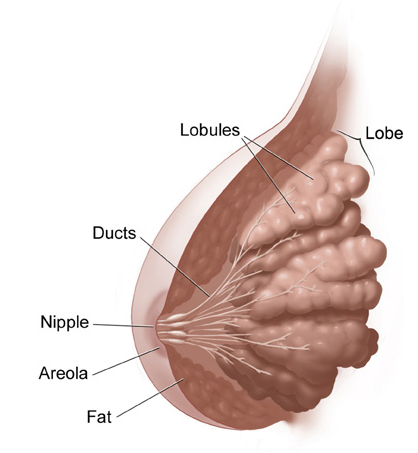
\includegraphics[width = 0.34\textwidth]{plots/breastAnatomy.png}
	\caption[Anatomy of the female breast]{Anatomy of the female breast. Image courtesy of~\cite{NCI2012}.}
	\label{fig:BreastAnatomy}
\end{figure}

The \emph{cancer stage} depends on the size of the tumor and whether the cancer cells have spread to neighboring tissue or other parts of the body. It is expressed as a Roman numeral ranging from 0 through IV; stage I cancer is considered \emph{early-stage breast cancer} and stage IV cancer is considered \emph{advanced}. Stage 0 describes non-invasive breast cancers, also known as \emph{carcinoma in situ}. Stage I, II and III describe invasive breast cancer, i.e., cancer has invaded normal, surrounding breast tissue. Stage IV is used to describe metastatic cancer, i.e., it has spread beyond nearby tissue to other organs of the body.

\subsection{Mammograms}
%\subsubsection{Mammograms}
A \emph{mammogram} is an x-ray image of the breast. Radiologists use \emph{screening mammograms} (normally composed of two mammograms of each breast) to check for breast cancer signs on women who lack symptoms of the disease. If an abnormality is found, a \emph{diagnostic mammogram} is ordered; these are detailed x-ray pictures of the suspicious region~\cite{NCI2014}. A standard mammogram is shown in Figure~\ref{fig:normalMammogram}.

\begin{figure}[h]
	\centering
	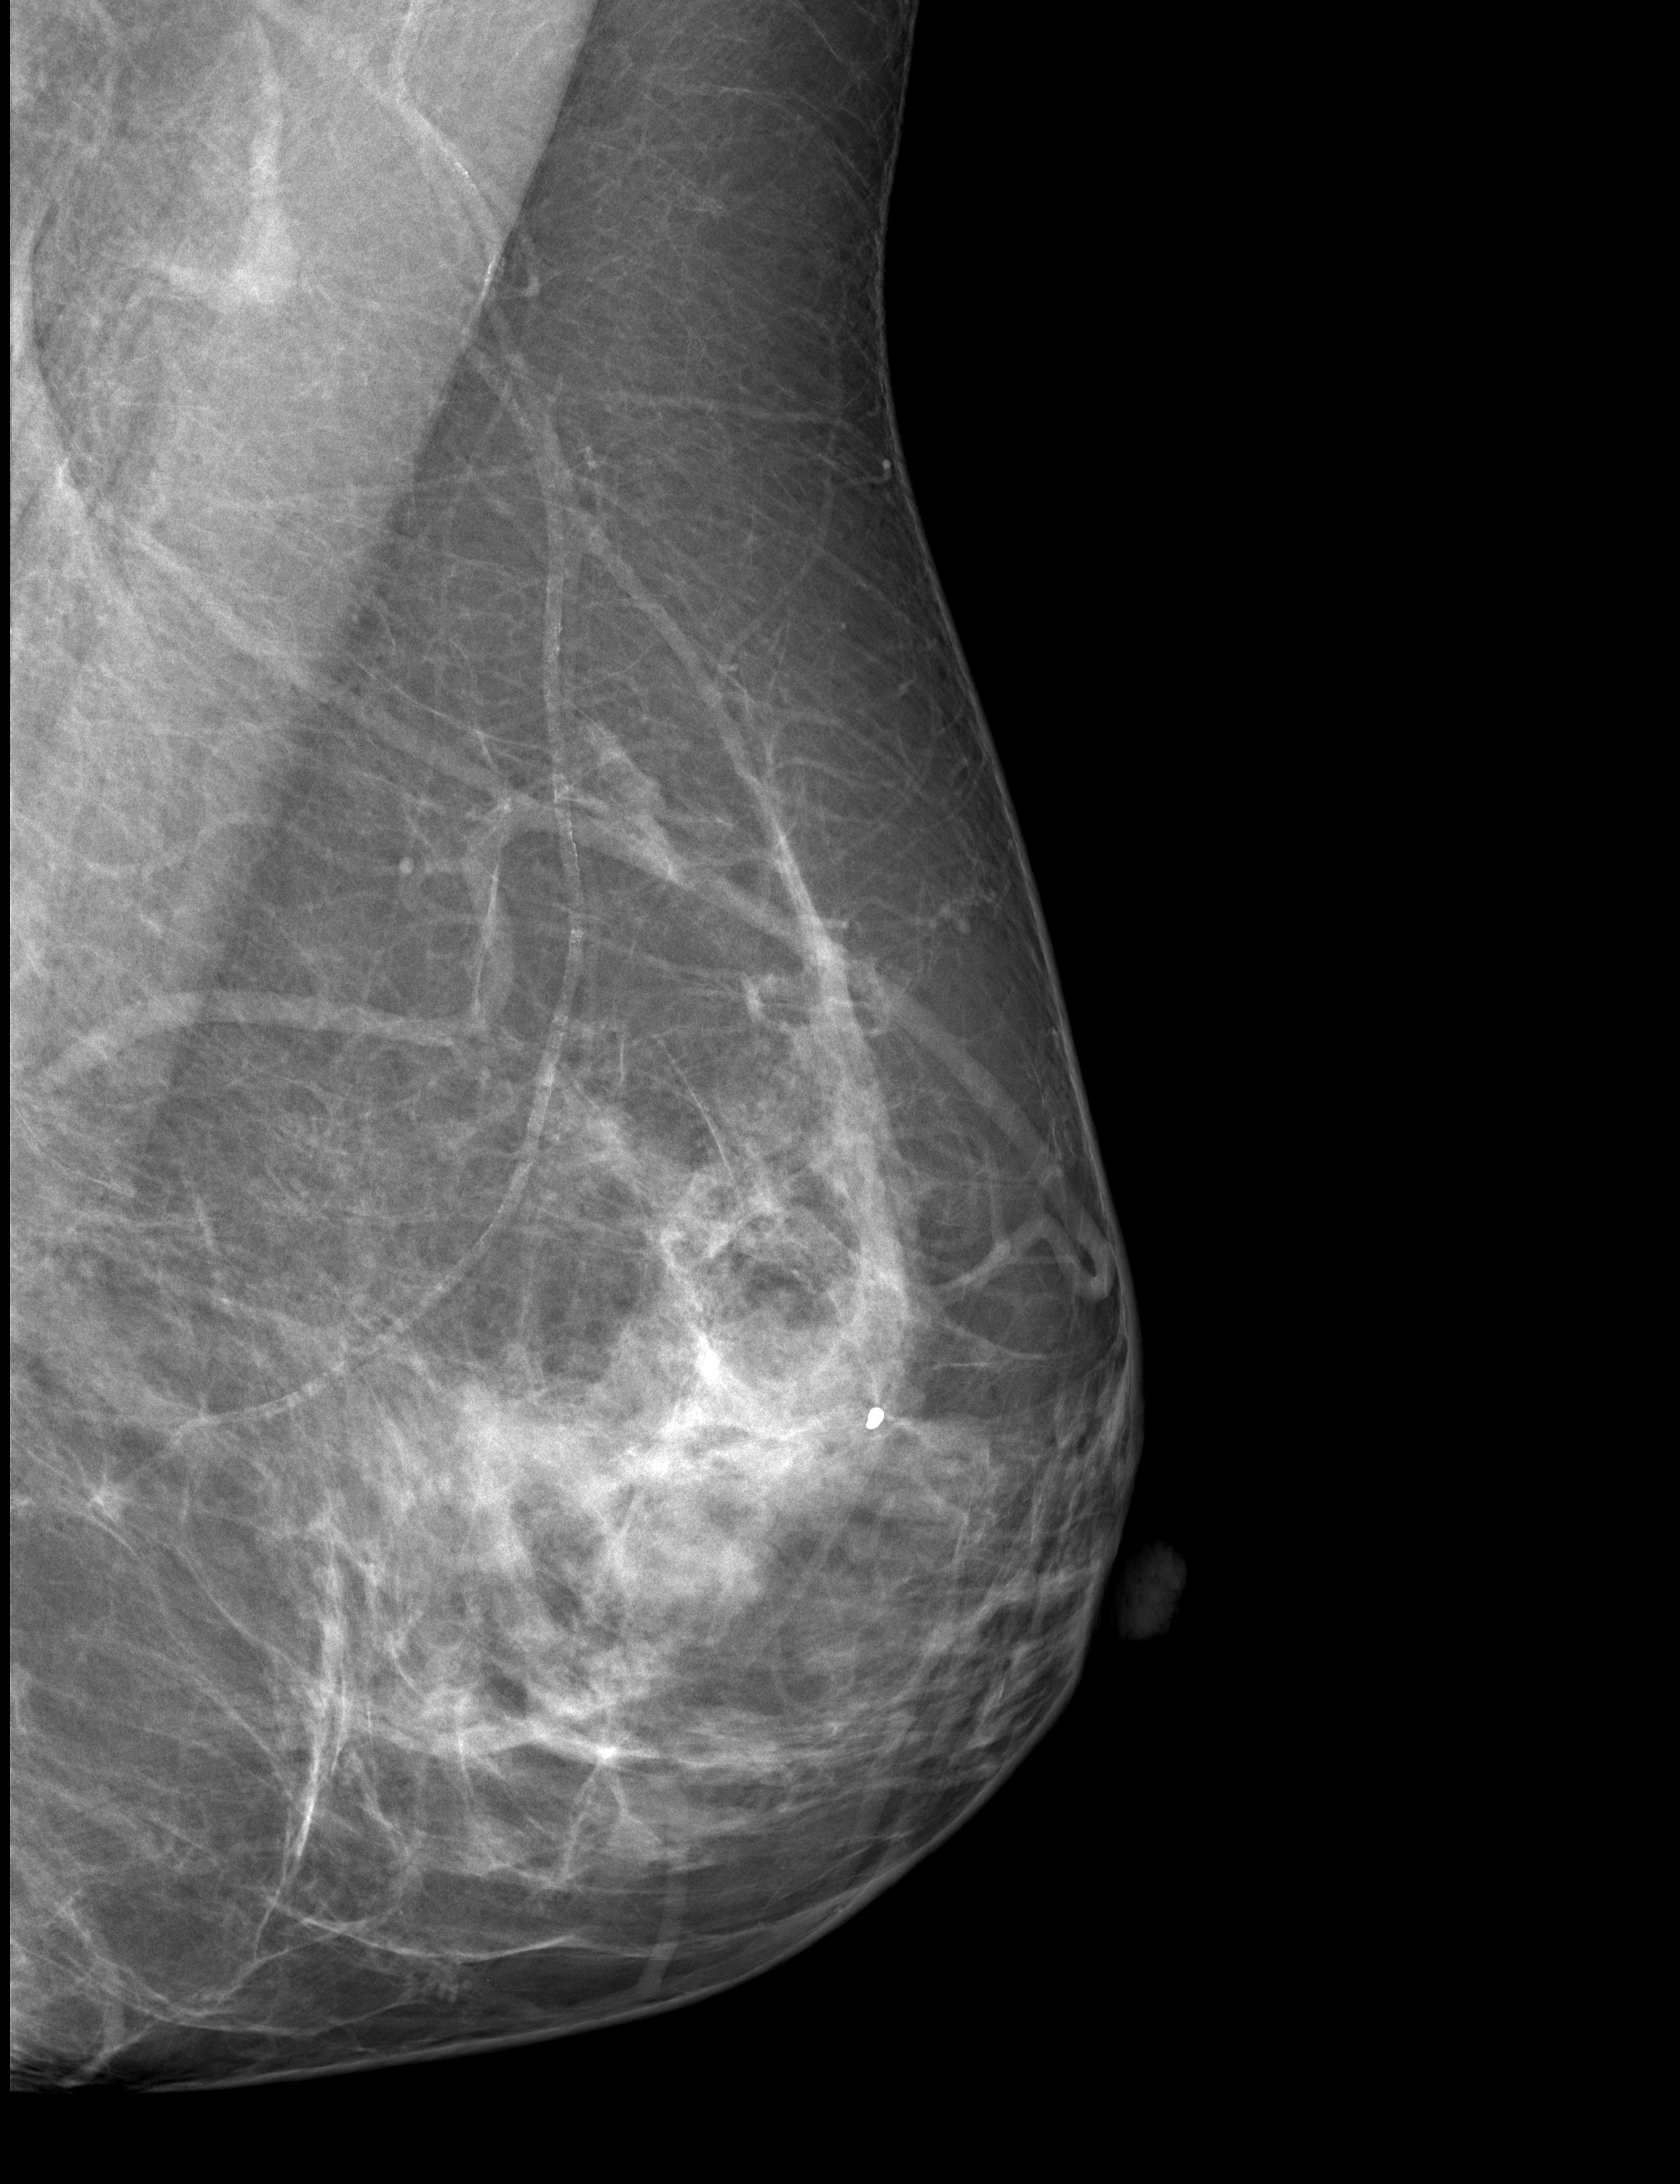
\includegraphics[width = 0.25\textwidth]{plots/normalMammogram.jpg}
	\caption[A digital mammogram]{A standard mammogram.}
	\label{fig:normalMammogram}
\end{figure}

Having a screening mammogram in a regular basis is the most effective method for detecting breast cancer early; around 85\% of breast cancers can be detected in a screening mammogram~\cite{BCSC2013}. Nevertheless, screening mammograms have many limitations: a high false positive rate, overtreatment in Stage 0 cancer, false negative results for women with high breast density, radiation exposure and physical and psychological discomfort~\cite{NCI2014}.

Radiologists look primarily for microcalcifications and breast masses. \emph{Microcalcifications} are tiny deposits of calcium in the breast tissue that can be a sign of early breast cancer if found in clusters with irregular layout and shapes (Fig.~\ref{fig:breastCancerSigns}). \emph{Breast masses} or breast lumps are a variety of things: fluid-filled cysts, fibric tissues, noncancerous or cancerous tumors, among others. A mass can be a sign of breast cancer if it has an irregular shape and poorly defined margins (Fig.~\ref{fig:breastCancerSigns}). Radiologists will also consider the breast density of the patient when reading a mammogram given that high breast density is linked to a higher risk of breast cancer~\cite{ACS2014}.
\begin{comment} My classification
Lesion
	Mass = Lump(This is palpable)
		Malignant = Cancerous
			Tumors
		Benign = Noncancerous
			Tumors
			Cysts
			Fibrosis/Fibroadenoma
	Microcalcifications (benign or malignant)

Tumors are abnormal growths of cells, cysts ae filled with fluid and fibrosis are "firmness in the connective tissues". Lesion is anything suspicious in a mammogram
Detection: Find lesions (malignant or benign)
Diagnosis: Find malignant lesions
\end{comment}

\begin{figure}[h]
	\centering
	\begin{subfigure}{0.24\textwidth}
                
\includegraphics[width=\textwidth]{plots/breastMicrocalcification.jpg}
        \end{subfigure}
	~
	\begin{subfigure}{0.24\textwidth}
                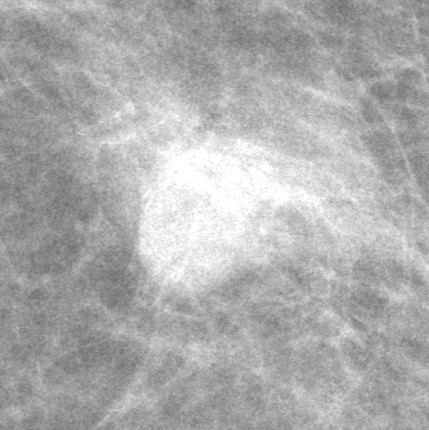
\includegraphics[width=\textwidth]{plots/breastMass.jpg}
        \end{subfigure}
	\caption[Signs of possible breast cancer]{Signs of possible breast cancer in a mammogram. Left: A cluster of microcalcifications in an irregular layout. Right: A poorly defined breast mass.}
	\label{fig:breastCancerSigns}
\end{figure}

%Conventional mammography uses film to record x-ray images of the breast. \emph{Digital mammography}, on the other hand, uses digital receptors that convert x-rays into electrical signals and stores the image electronically. 
Conventional mammography records mammograms in film; \emph{digital mammography}, on the other hand, converts x-rays into electrical signals and stores images electronically.
Digital mammograms offer a clearer picture of the breast and ease manipulation and sharing between health care providers.
% However, researchers still debate whether [[its|their] use over| they] [surpass| improve on|outperform|[offers|have] an advantage over|are more effective than|benefit] film mammograms [in|for] [identifying breast cancer|breast cancer detection].
Although researchers still debate whether they offer an advantage over film mammograms~\cite{Kerlikowske2011, Pisano2008, Skaane2007}, digital mammography has become standard in breast cancer screening. Figure~\ref{fig:normalMammogram} is, in fact, a digital mammogram.

\emph{Digital tomosynthesis} is a new technology that produces three-dimensional x-ray images of the breast and is expected to improve the efficacy of mammograms. Studies comparing the two techniques have not yet been published~\cite{NCI2014}.

\emph{Computer-aided detection (CAD)} systems assist radiologists during screening signaling suspicious areas and displaying relevant information. Detection or CADe looks for any type of lesion while diagnosis or CADx focuses on malignant lesions. Whether their use improves accuracy has been challenged~\cite{Lehman2015}.

% option: Delete this, downgrade mammograms to subsubsection and add the bcdr info in the solution/data set/database part. Maybe also leave the first paragraph in here as part of mammograms subsection, only change it to say "Mammography databases are important"
% option: do not add anything
\subsection{Mammographic databases}
%Databases are essential to mammographic image analysis;
%annotated
Researchers use data from previous patients---mammograms, segmentations and clinical features\textemdash to train and evaluate their models. 
%Databases offer pixel-wise labelled mammograms, lesions are segmented by expert radiologists.
%For this purpose, lesions are manually segmented to produce pixel-wise labels.
\emph{Contrast resolution}, the number of gray values per pixel, and \emph{spatial resolution}, breast area per pixel, dictate the quality of a digital mammogram: 12-bit images ($2^{12} = 4048$ gray values) with pixel size of at most 0.1mm are prefered. Many publicly available databases, including those described below, satisfy these conditions.

The Digital Database for Screening Mammography (DDSM)~\cite{Heath2001} is the most popular database used for CAD development. It is composed of around 10.5K digitized film mammograms from 2620 patients. Mammograms are either 12-bit or 16-bit images with 0.05 mm spatial resolution. Lesion segmentations are provided along with its type, assesment, subtlety and malignancy.%Patient data is also provided.
%Type is mass, microcalcification, assesment (1-5) in BIRADs, subtlety(1-5) and 

The BancoWeb database~\cite{Nepomuceno2011} consists of around 1.5K digitized film mammograms from 300 Brazilian patients. Mammograms are 12-bit images with 0.075 or 0.15 mm pixel size. Although few lesions are segmented, this repository may be useful to assess performance in Latin American patients. Its current state is unknown.

Lastly, the Breast Cancer Digital Repository (BCDR-DM)~\cite{Moura2013a, Moura2013b} consists of around 1.2K digital mammograms from 237 patients. Mammograms are 8-bit images with 0.07mm spatial resolution.
Lesion segmentations are provided as well as their assesment, hand-crafted texture and shape features and relevant clinical data.
%It provides lesion segmentations and assesments, hand-crafted texture and shape features and relevant clinical data

\begin{comment}
Another small digital mammogram repository is called INbreast~\cite{Moreira2012}. It consists of 410 digital mammograms from 115 patients. Each mammogram is a 14-bit image with 0.7 mm spatial resolution. Lesion boundaries are accurately marked and its information is also included. This could be used in conjunction with the BCDR-DM repository.

Finally,~\cite{Zheng2012} used a private repository of around 6.5K digital mammograms obtained from 1120 patients. Specifics of contrast and spatial resolution are not provided but they are most probably good enough. Lesions are marked (with a circle) on the mammograms and lesion and patient information is provided. Even though this is a private repository of the University of Pittsburgh, if needed, we could ask them for access to it. This may not be plausible given the complications of sharing personal (granted anonymized) information and the size of the database.
\end{comment}

This section was written using information from the National Cancer Institute. We recommend to visit its website (\url{www.cancer.gov}) for further details.


	\subsection{Mammography DB}
	\label{subsec:MammographyDB}

	\subsection{Classification}
	\label{subsec:Classification}
	%\emph{Machine learning} is the study of algorithms that create models (either of a population or of a function of interest) and estimate their parameters from data  in order to make good predictions or inferences.
%Machine learning is the study of mathematical models either of a population or of a function of interest and the algorithms used to estimate their parameters from data in order to make predictions or inferences.
\emph{Machine learning} is the study of algorithms which build models of a population or a function of interest and estimate their parameters from data in order to make predictions or inferences. A machine learning expert knows how to choose the right model for the problem in hand (\emph{model selection}), how to efficiently estimate its parameters from the available data (\emph{learning} or \emph{training phase}) and how to evaluate the trained model (\emph{testing phase}).

Machine learning problems can be divided into three categories depending on the data used to train the model: \emph{supervised learning}, where we learn a function $f(x)$ using a set of examples which are labelled with the correct output, for instance, learning a function that estimates the price of a house given its size and number of bedrooms from a dataset of houses labelled with their real value; \emph{unsupervised learning}, where we look for relationships and structure in unlabelled data, for instance, given a dataset of potential customers find those who are likely to buy a car and \emph{reinforcement learning}, where the only feedback received are rewards, for example, learning to play tetris from a dataset of world states and actions and where rewards are received sparsely every time points are earned (when lines dissapear). Supervised learning can be further divided in regression and classification. If the expected output is numerical, e.g., the price of a house, it is called \emph{regression}, if the expected ouput is categorical, e.g., spam or no spam, it is called \emph{classification}. We will focus on classification.

A \emph{classifier} takes as input a vector of \emph{features} $x \in \mathbb{R}^n$ from a problem instance and produces an \emph{output} $h(x)$ predicting the class $y$ that instance belongs to, i.e., it concretely models the underlying function $f(x)$ as $h(x)$ ($h$ stands for hypothesis). \emph{Binary classification}, when $y$ can only take two values e.g., cancer/no cancer, is the most common kind of classification and \emph{multiclass classification}, when $y$ can take $K > 2$ different values, can be performed by using $K$ binary classifiers. Some classifiers, such as convolutional networks (defined in Section~\ref{subsec:ConvNets}, output a \emph{score vector} $h(x) \in \mathbb{R}^K$ where $h(x)_k$ is a measure of the probability that $x$ belongs to class $k$. Every classifier partitions the \emph{feature space}, the $n$-dimensional space where features exist, into separate \emph{decision regions}, regions of the space which are assigned the same predicted outcome; a \emph{decision boundary} is the hypersurface that partitions the feature space. Classifiers are sometimes classified as \emph{linear} or \emph{nonlinear} according to the nature of the decision boundary they impose on the feature space. Logistic regression, for instance, is a linear classifier while an artificial neural network (with at least one hidden layer) is nonlinear.
% A linear classifier can separate perfectly linear data, while for nonlinear data a more powerful classifier is needed. Linearly separable data are those which can be classified by a linear classifier while nonlinear data can not.

The \emph{loss function} $J(\theta)$ of a classifier measures the amount of error the classifier incurs in for a particular choice of parameters $\theta$. There are various ways to formulate this function. A \emph{least-squares loss function} for a binary classifier (such as logistic regression) is presented in Equation~\ref{eq:LossFunction}
\begin{equation}
	J(\theta) = \frac{1}{2m}\sum_{i=1}^m(h_\theta(x^{(i)}) - y^{(i)})^2
	\label{eq:LossFunction}
\end{equation}
where $m$ is the number of training examples, $y \in \{0,1\}$ is the real class of the example $x$ and $h_\theta(x) \in \mathbb{R}$ is the output of the classifier for input $x$ with parameters $\theta$, this represents the probability that $x$ belongs to the positive class 1. We introduce another (rather more complex) loss function in the next section.

A classifier is trained by choosing the parameters $\theta$ that minimize its loss function, hence, minimizing the expected error of the classifier on the training set. \emph{Gradient descent} is a method used to estimate the parameters that minimize $J(\theta)$: at the start, it initializes parameters at random and iteratively updates each parameter using the gradient of the loss function until it converges to a minimum. Specifically, at each iteration it performs the update:
\begin{equation}
	\theta = \theta - \alpha \nabla{J(\theta)}
\end{equation}
where $\alpha$, called the \emph{learning rate}, defines the step size. Gradient descent is guaranteed to converge to a global minimum if the loss function is convex, convexity of the loss function depends on the model $h(x)$.

To select the best model $h(x)$ for a particular problem or equivalently to select the best classifier for the problem each model is trained on a subset of the data set and later evaluated on a disjoint subset. In the {validation set approach} the data set is split into a training set (usually 70-90\%) and a validation set, each model is trained using the training set and evaluated on the validation set and the model which shows the best performance is selected. \emph{k-fold cross validation}, on the other hand, divides the data set in $k$ disjoint subsets (usually 5 or 10) and uses $k-1$ subsets to train the model and the remaining subset for evaluation, this process is repeated $k$ times for each model leaving out a different subset each time and the $k$ performance measures are averaged to obtain a final measure for the model.
%Cross validation produces better error estimates but is computationally costly.
\emph{Model hyperparameters}, settings which modify the underlying model or learning algorithm, are selected in the same way.

The model representation $h(x)$ needs to be chosen carefully. If we have an overly \emph{flexible} model, i.e, $h(x)$ is a complex function with many parameters to be learned compared to the size of the training set, the classifier will probably \emph{overfit} the data, this means that the parameters are fitted way too closely to the data and will pick up every small fluctuation and noise in the training set causing the trained classifier to produce almost perfect results on the training set but perform poorly on previously unseen examples. The opposite is also true, when $h(x)$ is very simple the classifier lacks the power to model the function of interest and we say that it \emph{underfits} the data. This problem is sometimes referred as the \emph{bias-variance tradeoff}. A high variance classifier is prone to overfitting, while a high bias classifier is prone to underfitting.

A popular way to avoid overfitting (and underfitting) is to use a flexible model trained with regularization. \emph{Regularization} modifies the loss function to include a penalty to the complexity of the model, thus forcing the learning stage to choose parameters that minimize both the training error of the classifier and the complexity of the model. Equation~\ref{eq:l2NormRegularization} shows the least-squares loss function with \emph{$l_2$-norm regularization}:
\begin{equation}
	J(\theta) =  \frac{1}{2m}\sum_{i=1}^m(h_\theta(x^{(i)}) - y^{(i)})^2 + \frac{\lambda}{2m} ||\theta||_2
	\label{eq:l2NormRegularization}
\end{equation}
where $||\cdot||_2$ is the euclidean norm of a vector. In addition to reducing training error, minimizing the regularized loss function will shrinken the parameters $\theta$ hopefully setting some of them to zero, thus simplifying $h(x)$. The \emph{regularization strength} $\lambda$ regulates the tradeoff between less training error and less regularization error. \emph{$l_1$-norm regularization} or \emph{lasso} is similar to $l_2$-norm regularization except that it shrinks the $l_1$-norm of $\theta$ instead of the $l_2$-norm.

To evaluate the performance of a classifier we use a separate set of examples (a test set) which should have not been used for training or validation. Classification accuracy is the standard performance measure in machine learning. \emph{Accuracy} measures the proportion of test set examples which are correctly classified. Its compliment, \emph{error rate}, measures the proportion of test set examples which are incorrectly classified. Accuracy, nonetheless, is not a good evaluation metric for unbalanced data sets, data sets which have many more examples of one class than the other e.g., cancer data sets are often unbalanced as most examples belong to the negative class (no cancer) than the positive class (cancer). For instance, a classifier which always predicts no cancer regardless of the input will show a high accuracy (equivalently a low error rate) even though it is not a good model for the problem.

A different set of metrics based on the confusion matrix of the classifier are used to evaluate its quality in unbalanced data sets. A \emph{confusion matrix} is a matrix which summarizes the results of a classifier in the test set (see Table~\ref{tab:ConfusionMatrix}).
\begin{table}[h]
	\centering
	\begin{tabular}{cc|c|c|}
		&\multicolumn{3}{c}{\textbf{Actual class}}\\
		&&Positive & Negative \\
		\cline{2-4}
		\textbf{Predicted}&Positive&True Positives (TP)& False Positives (FP)\\
		\cline{2-4}
		\textbf{class}&Negative&False Negatives (FN) & True Negatives (TN)\\
		\cline{2-4}
	\end{tabular}
	\caption{Confusion matrix for a binary classifier}
	\label{tab:ConfusionMatrix}
\end{table}
\emph{True positives} is the number of positive examples which were correctly predicted as positive. \emph{False positives} is the number of negative examples which were incorrectly predicted as positive. True negatives and false negatives are defined in a similar fashion. Based on the confusion matrix we can compute some commonly used metrics:
\begin{equation}
	Sensitivity \text{ or } Recall = \frac{TP}{TP+FN}
\end{equation}
\begin{equation}
	Specificity = \frac{TN}{FP+TN}
\end{equation}
\begin{equation}
	Precision = \frac{TP}{TP+FP}
\end{equation}
Sensitivity and specificity are usually preferred to present results in medical diagnosis meanwhile precision and recall are preferred in machine learning. \emph{Sensitivity} measures the proportion of positive examples predicted as positive and \emph{specificity} measures the proportion of negative examples predicted as negative. \emph{Precision} is a measure of the proportion of examples predicted as positive which are actually positive. A good classifier will have both high sensitivity and high specificity or similarly, high precision and high recall. It is always useful to have a single metric to evaluate classifiers, for example, to choose between two models; we show two commonly used metrics in Equation~\ref{eq:F1Score} and~\ref{eq:G-mean}.
\begin{equation}
	F_1\text{ }score = 2\times\frac{Precision \times Recall}{Precision + Recall}
	\label{eq:F1Score}
\end{equation}
\begin{equation}
	G\text{-}mean = \sqrt{Sensitivity \times Specificity}
	\label{eq:G-mean}
\end{equation}

In this thesis, we will generally present results for all this metrics (precision, recall or sensitivity, specificity, $F_1$ score and G-mean). The metric used when selecting a model influences its characteristics and behaviour, hence, one should put some consideration into choosing it. We favor $F_1$ score over G-mean because it concentrates on prediction in the positive class (cancer) which is harder to predict and the class we are more interested in. Furthermore, it represents a more balanced tradeoff (an small change in precision is corresponded with a small change in recall) than G-mean where an small change in specificity can be corresponded with a big change in sensitivity.
\begin{comment} Discussion of why G-mean over F1
(Not sure about this) As a rule of thumb, using G-mean will generate models that predict more positives given that the sensitivity will greatly improve and specificity will only slightly decrease. Using $F_1$ score, the model will predict less positives as that will improve precision but only slightly decrease sensitivity. 

Why G-means? Because it is more important to obtain a low error in specificity than in precision, i .e, would you prefer a 90% in specificity or a 90% in precision?. 90% in specificity means that 10% of actual negatives (10 persons) were told they have no cancer although they actually had cancer, meanwhile 10% of expected positives(a small number, maybe 1) was said he has cancer although he doesn{t. First is worse.

Using G-mean i will predict more positives, no matter what. My sensitivity is going to vastly improve and the specificity will only decrease a little, but the precision is gonna take a hit. Because if I predict less positives sensitivity is gonna go down, specificity is gonna go up (as I add more true negatives) but just a little and precision  would go up (but it wouldn't matter for g-mean).

Using F1 I'll probably predict less positives, sensitivity is going to go slightly down, and precision is going to go up, specificity doesn{t matter but it will decrease a little. Or I'll probably predcit as many poositives as needed. It focuses more on the positive class.

Other diagonal, the algorithm will learn negatives pretty well, so the one that predicts less positives(f1) probably isn{t learning much (it is predicting all negative).
\end{comment}

This section is meant to be a compendium of basic concepts in machine learning, practical machine learning involves many subtleties and implementation details not mentioned here. Notation and content in this section is mostly based on materials from Stanford's Machine Learning course\cite{Ng2014}.


	\subsection{Artificial Neural Networks}
	\label{subsec:ANNs}

	\subsection{Convolutional Networks}
	\label{subsec:ConvNets}

	\subsection{Convolutional Networks applied to Breast Cancer}
	\label{subsec:BreastCancerConvNets}	

	\subsection{Related Work}
	\label{subsec:RelatedWork}
	In this section we offer a summary of some of the first work on using convolutional networks for breast cancer diagnosis as well as some of the articles that have influenced this thesis.

Lo et al.\cite{Lo1995} were the first group to use convolutional networks for breast cancer detection. They used a CNN with two hidden layers to detect microcalcifications. A high sensitivity image processing technique was used to obtain a set of 2104 patches (16 by 16 pixels) of all potential disease areas from 68 digital mammograms; of these, 265 were true microcalcifications and 1821 were ``false subtle microcalcifications". Prior to training the CNN, a wavelet high-pass filtering technique was used to remove the background of these images. Each image was flipped over (left-right) and 4 rotations for each the original and flipped images were used for training (0°, 90°, 180° and 270°). The CNN was composed of one input unit ($16\times16$), 12 units in the first hidden layer ($12\times12$), 12 units in the second hidden layer($8\times 8$) and two output nodes(one for YES and one for NOT). The input size ($16\time16$), number of hidden layers ($2$) and kernel size ($5\times5$) was obtained via cross validation, altough not many other options were explored: they tried input sizes of 8, 16 or 32, one or two hidden layers and kernel sizes of 2, 3, 5 or 13. The CNN reached 0.87 average AUC when identifying individual microcalcifications and 0.97 AUC for clustered microcalcifications. Only a minimum of three calcifications was considered a detection. Sensitivity and specificity test results were not reported. This article proved that simple convolutional networks can be efficiently used for medical image pattern recognition.
%Lesson learned: two hidden layer newtwork produces better results, background reduction is neccesary and using matrices invariance to augment the data helps. Convnets work helps and convnets work.

%A refined approach was presented some years later by the same authors along some non convolutional neural networks~\cite{Lo1998}. The setting is very similar but ..... Results are..

%work done at Tec


\section{Methodology}
In order to achieve the proposed objectives and test our hypotheses we will need to carry out various tasks. We list them here in the order in which we plan to execute them: %although some steps could be executed simultaneously:

\begin{itemize}
	\item Literature review: A thorough review of the published work using the databases and resources available in the institution. By the end of this task, a complete theoretical background should be obtained and written. This will also help refine the scope of the project and the experiments to be conducted.
	\item Software review: Once a clear idea of what are the possible experiments to be executed, we will need to find appropiate software to perform them. Software for database managing, preprocessing and implementation of different neural networks should be either located or developed.
	\item Database preprocessing: We will ready the database images for the experiments; these implies joining different databases, obtaining the required features, preprocessing the images, assigning labels, etc.
	\item Assesing image preprocessing: We will train a standard convolutional network with fixed parameters on mammograms with three different preprocessings: no preprocessing, image enhancement using median or gaussian filters and wavelet filtered images. Furthermore, we will train a deeper convolutional network on nonpreprocessed images. We want to answer three research questions: which is the best preprocessing for convolutional networks, is using the best filter significantly better than using nonpreprocessed images and can a convolutional network automatically preprocess the images?
% Q: Is it better to make different preprocessings oin the same convolutional network or to fit each convolutional network for each preprocessing, thus, giving it the best chance to perform but taking more time.
	\item Exploratory experiments: We will train standard convolutional networks in two different inputs: small image patches obtained from mammograms and whole mammogram images. We will also train a linear classifier, probably rectified linear units, on the features obtained from a convolutional network trained on the ImageNet database, i.e., we will use an already trained convolutional network instead of one trained specifically in mammograms. Here we will use the image preprocessing technique that showed better results in the previous step. We want to answer two research questions: Can a convolutional network trained on whole mammograms perform as well as one trained on small patches and can we use an already trained convolutional network to classify mammograms?
	\item Model selection: Using the insights from previous sections and the current literature on convolutional networks, we will select a network architecture along with novel features, preprocessing, training and regularization procedures. We aspire to find the best convolutional network configuration for mammogram classification.
	\item Further experimentation: We will train the chosen convolutional network on our mammographic database. We will perform crossvalidation to adjust the most important network parameters and use regularization to avoid possible overfitting. We want to answer two research questions: is the performance of the convolutional network considerably improved by parameter tuning and, more importantly, is this a good performance?.
%Maybe train one with no tune fitting.
	\item Gathering results: Produce results on the test set and elaborate figures and tables. This could be obtained directly from software output or from further program executions.
	\item Reporting results: Write the thesis and any article or technical guide which may result from this work. Both this and the previous step will be performed along the execution of the project, hopefully benefiting from the supervisors' feedback.
\end{itemize}
Finally, we want to note that this is an idealized workflow and some changes may occur due to time limitations or resources unavailability. In the unlikely case that the work is finished before the project deadline, we will either reiterate on model selection, experiments, result gathering and reporting or look into digital tomosynthesis, network ensembles or evolving convolutional networks.

\begin{comment}
La {\it Metodología} (o lo que algunos autores llaman el {\it Método})
 es el proceso o
conjunto de pasos que debe efectuarse para llegar a cumplir con los
objetivos. Esos pasos deben contener  los experimentos a realizar, la forma de
llevarlos a cabo, la evaluación de los resultados, la prueba de las hipótesis,
la respuesta a las preguntas de investigación y el último paso debe ser el
reporte escrito de los resultados.
\end{comment}


\section{Work Plan}
Yet to write

\begin{comment}
Una vez establecida la {\it Metodología} es importante establecer las
actividades con sus tiempos respectivos en lo que se llama el {\it Plan de
Trabajo}. Ello nos da una idea clara de la extensión en tiempo del trabajo
propuesto. Además de ser necesario, lo cual es normalmente cierto en
propuestas de proyecto industrial, es importante establecer el PLAN FINANCIERO
el cual desglosa los recursos necesarios para el desarrollo del proyecto y sus
costos.

{\bf Un ejemplo de Plan de Trabajo}

La figura \ref{ttphd} presenta el cronograma de las actividades que llevarán a
cabo los objetivos de esta tesis. 

\begin{figure}[th]
	\centerline{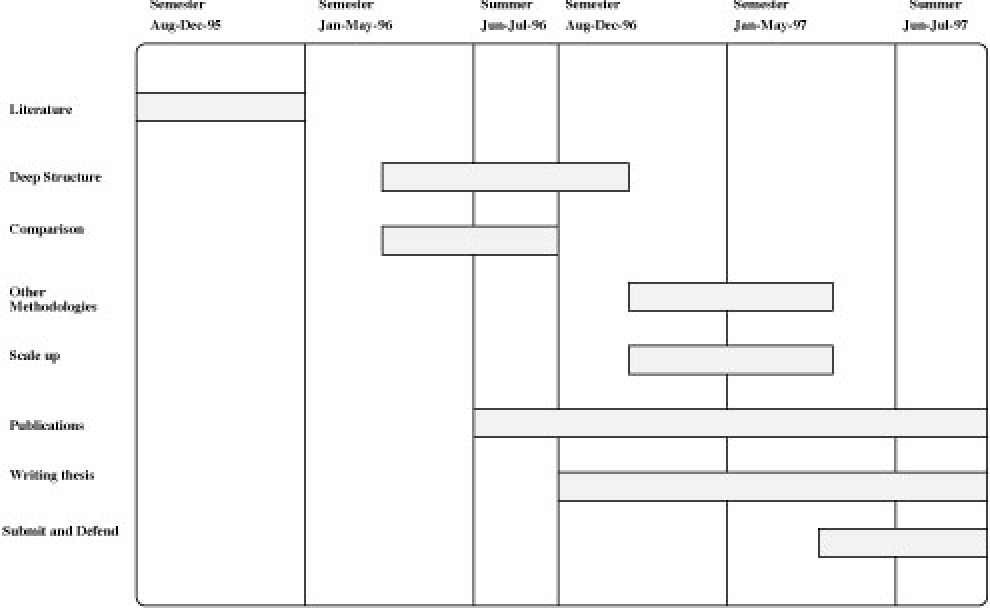
\includegraphics[width=4in,height=3in]{plots/ttphd.pdf}}
	\caption{Cronograma de Actividades para desarrollar la Tesis}
	\label{ttphd}
\end{figure}
\end{comment}


% Bibliography
\bibliographystyle{apalike}
\bibliography{bibliography}

\end{document} 
